\chapter{Project budget}
This chapter details the budget associated to the development of this research project. For this, we will take into account the costs of the time invested on research, development and documentation writing, along with other indirect costs associated to the project activities.

\section{Gantt chart}
Figure \ref{gantt_chart} shows a Gantt presenting the different stages of the project and the distribution of time between them. As we can observe in the figure, the project can be divided into three main sections:
\begin{itemize}
\item Preliminary research on previous work.
\item Development of each rootkit module.
\item Documentation.
\end{itemize}

It is relevant to note that in this research work, because of the complexity and variety of functionalities of the eBPF system, each of the offensive capabilities of eBPF has been discovered and implemented as a rootkit module individually. Therefore, there has not existed a single iteration of analysis, design and implementation, but rather multiple iterations have been made to develop each module. This is the reason why, if we focus our view in the development stages, each consists on at least one analysis and multiple design and implementation activities.


\begin{figure}[htbp]
	\centering
	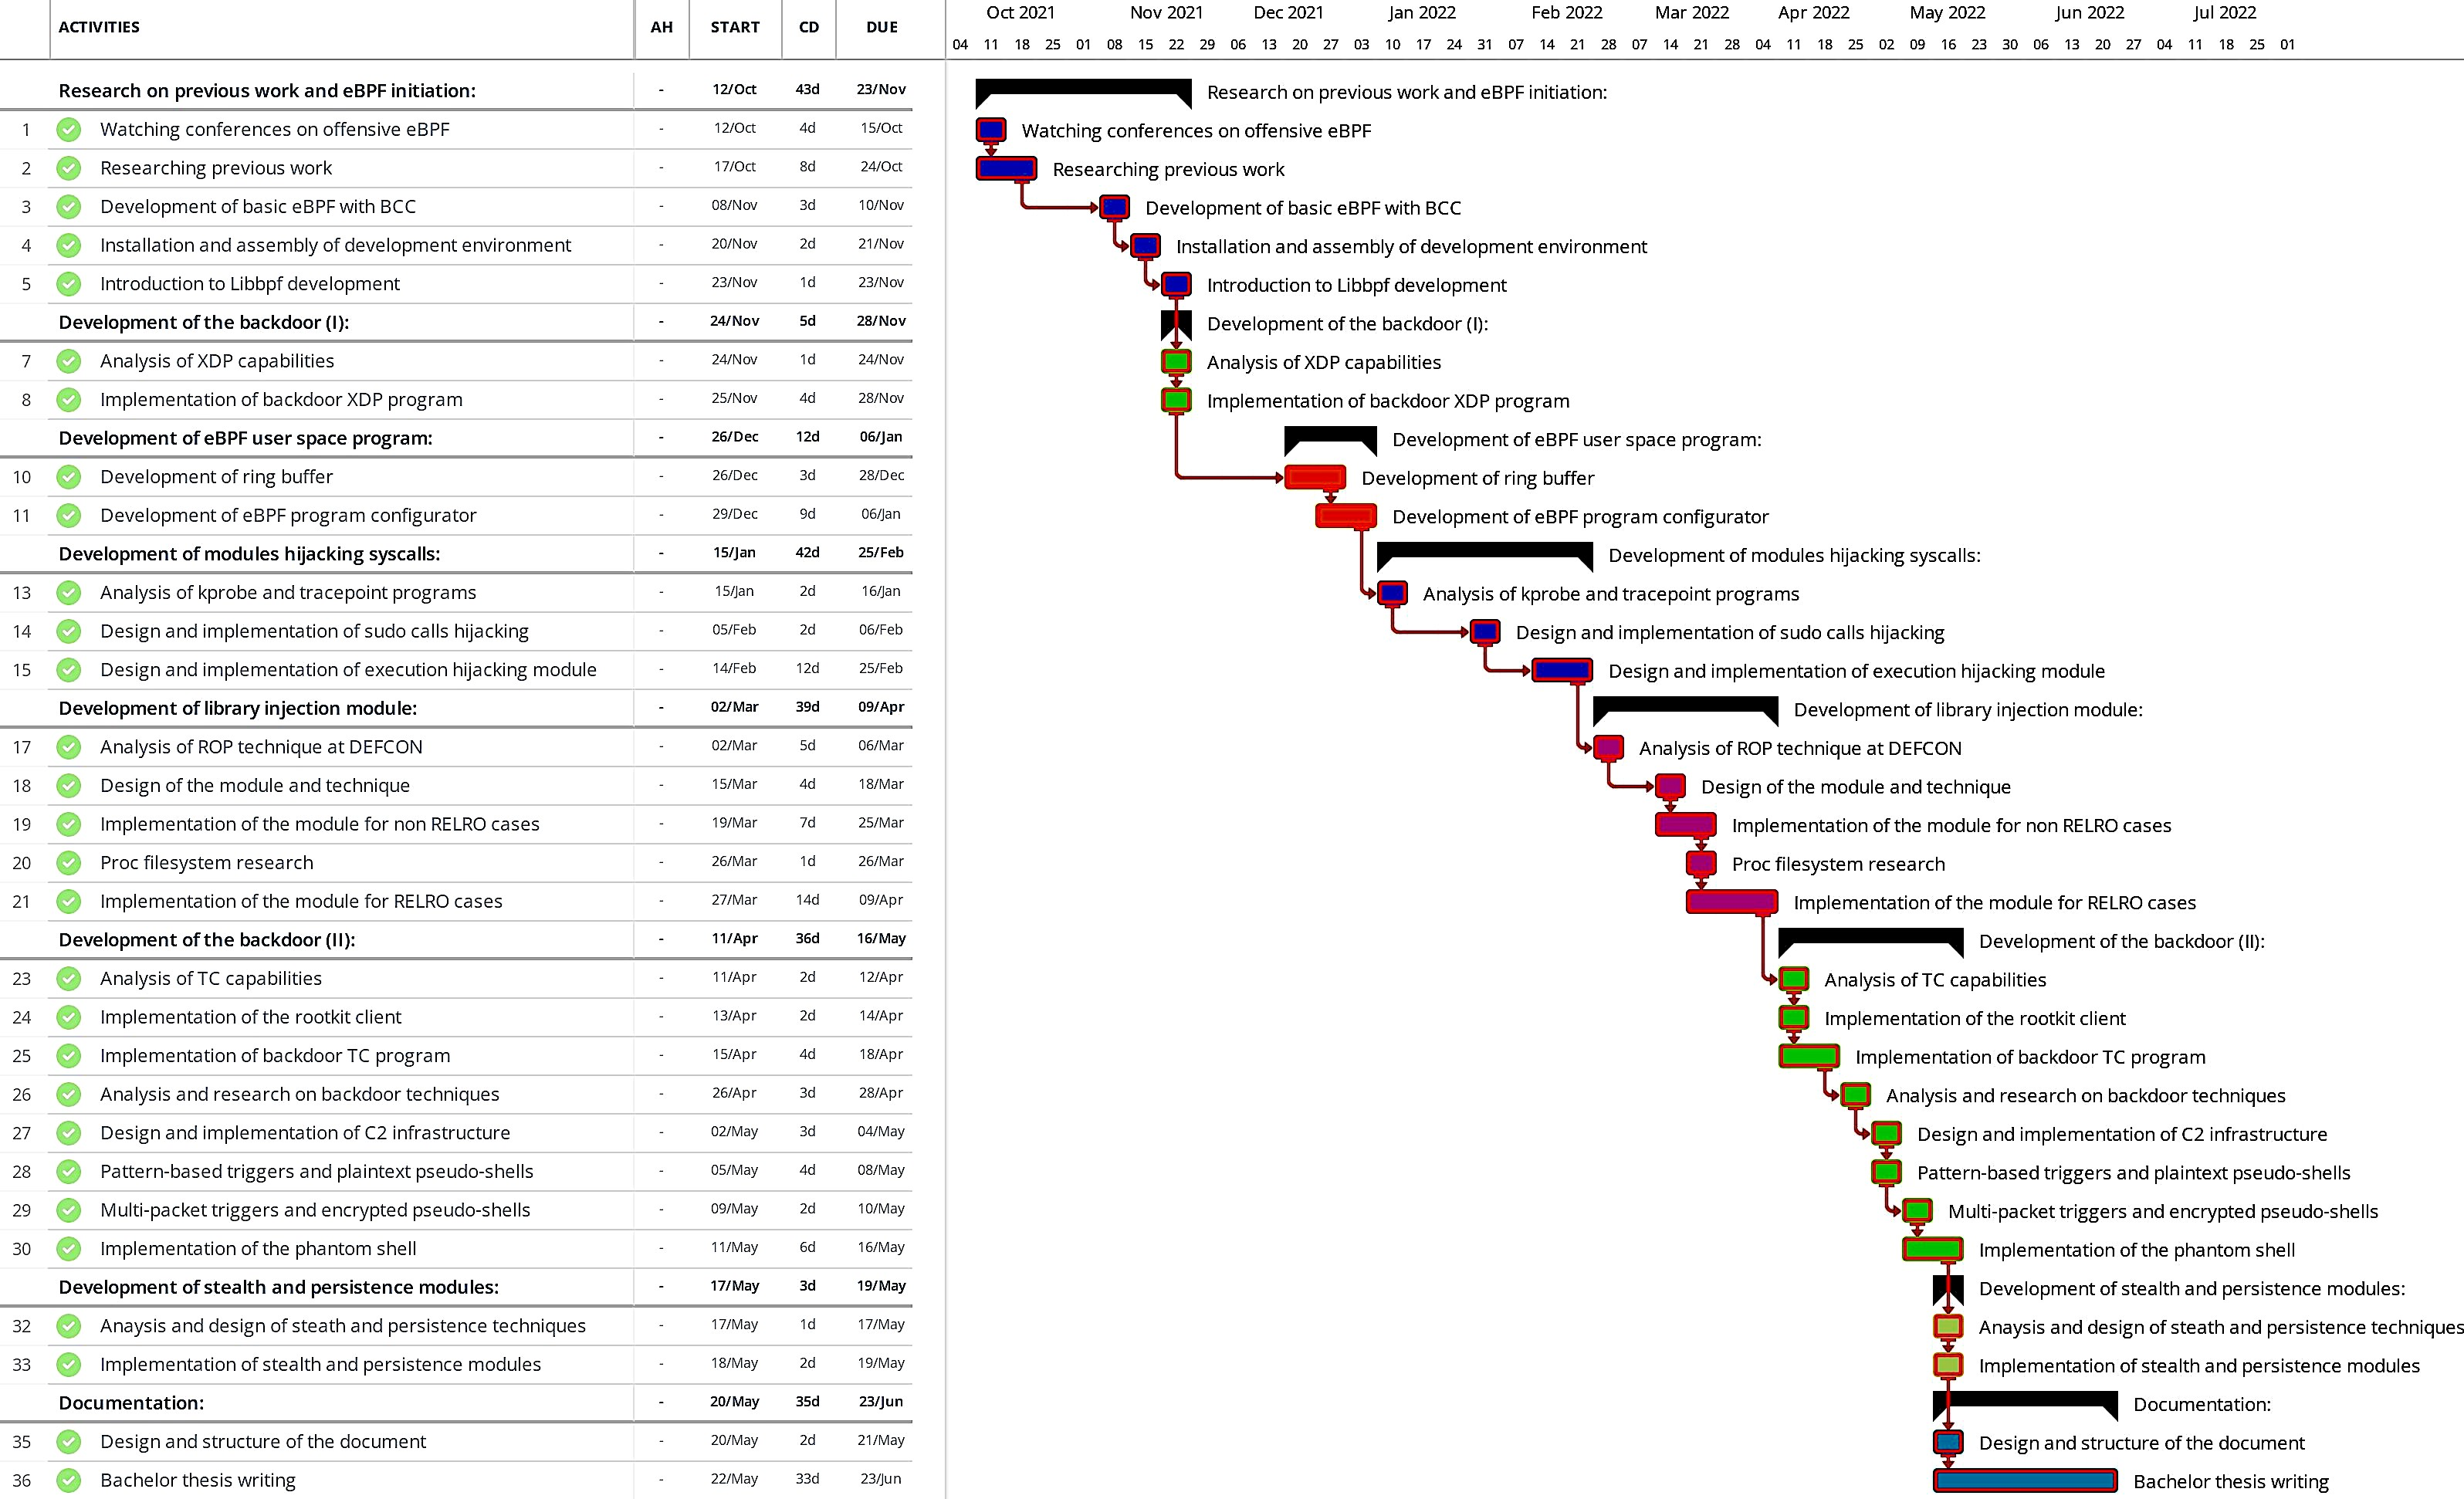
\includegraphics[width=15.4cm]{gantt_chart.jpg}
	\caption{Execution of simple\_timer.c with rootkit active.}
	\label{fig:gannt_chart}
\end{figure}

\section{Estimated costs}
This section presents an estimation of the costs associated with the  personnel conducting the activities described in the Gantt chart in addition to all costs derived from the development of this work.

\subsection{Personnel costs}
Although this project has been developed individually under the supervisor guidance, we can identify three different roles:
\begin{itemize}
\item A \textbf{cyber security analyst}: a role requiring expertise and knowledge about multiple aspects of Linux systems (such as ELFs, memory architecture and attacks at process memory), needed for identifying possible offensive capabilities of eBPF. Therefore this role is responsible of research and analysis of the offensive capabilities of eBPF. It will also write the corresponding documentation with the gathered knowledge.
\item A \textbf{programmer}: a role requiring knowledge about C programming and, preferably, eBPF developing experience (which requires a different skillset than normal C, being more similar to the development of programs for the Linux kernel).
\item A \textbf{project manager}: a role which administers the tasks and objectives to complete, contributing leadership and guidance to the team.
\end{itemize}

We will now consider the wages assigned to each role. The monthly and hourly salaries are displayed on Table \ref{table:salary_personnel}, and have been obtained using the salaries shown by Glassdor for each role in the city of Madrid \cite{glass_analyst} \cite{glass_manager} \cite{glass_programmer}. We have also assumed that these roles correspond to full-time positions consisting of 40 hours a week, 8 hours a day, with no vacations.

\begin{table}[htbp]
\begin{tabular}{|c|c|c|}
\hline
\textbf{ROLE} & \textbf{MONTHLY RATE} & \textbf{HOURLY RATE}\\
\hline
\hline
Cyber security analyst & 26424 € & 12.70 € \\
\hline
Programmer & 27018 € & 13.00 € \\
\hline
Project manager & 40000 € & 19.23 € \\ 
\hline
\end{tabular}
\caption{Average monthly and hourly salary for project staff.}
\label{table:salary_personnel}
\end{table}

Given the different responsabilities of the team members on the project, table \ref{table:hours_personnel} shows the number of hours which each person dedicates daily  to the project in average when perfoming each of the tasks (that is, the length of a working day when assigned to each task). 

Also, note that our own RawTCP\_Lib library is a relevant part of this project but it has been developed outside of the scope of this research. Therefore, we will consider it as an estimated 20-days long 4 hours/day development by the programmer.

\begin{table}[htbp]
\begin{tabular}{|c|c|c|}
\hline
\textbf{ROLE} & \textbf{TASK} & \textbf{HOURS/DAY}\\
\hline
\hline
\multirow{2}{*}{Cyber security analyst} & \multicolumn{1}{c|}{Research and analysis} & \multicolumn{1}{c|}{5}\\
\cline{2-3}
& \multicolumn{1}{c|}{Documentation writing} & \multicolumn{1}{c|}{10} \\
\hline
\multirow{2}{*}{Programmer} & \multicolumn{1}{c|}{Rootkit implementation} & \multicolumn{1}{c|}{7} \\
\cline{2-3}
& \multicolumn{1}{c|}{RawTCP\_Lib development} & \multicolumn{1}{c|}{4} \\
\hline
Project manager & Supervision and guidance & 1.16 \\ 
\hline
\end{tabular}
\caption{Daily dedication, in hours, that each personnel member needs to dedicate to each of their tasks.}
\label{table:hours_personnel}
\end{table}

With respect to the project manager, whose supervision task was not shown in the Gantt chart, we have considered an estimate of a total of 250 hours worked over the 215 days long project, dedicating an average of 8.18 hours once every week, or 1.16 hours daily.

With these salaries and work hours in mind, the tasks described on the Gantt chart are then distributed among these roles, as shown in Table \ref{table:personnel_total}. The total salary is calculated by taking into account the hourly salary of each role and the number of hours worked on each task (the product between hours in a working day and the total number of days).

\begin{table}[htbp]
\begin{tabular}{|>{\centering\arraybackslash}p{3cm}|c|>{\centering\arraybackslash}p{3cm}|c|}
\hline
\textbf{ROLE} & \textbf{TASK} & \textbf{DEDICATION} & \textbf{TOTAL}\\
\hline
\hline
\multirow{2}{*}{\shortstack{Cyber security\\ analyst}} & \multicolumn{1}{c|}{Research and analysis} & \multicolumn{1}{c|}{27 days} & \multirow{1}{*}{1714.50 €}\\
\cline{2-4}
& \multicolumn{1}{c|}{Documentation writing} & \multicolumn{1}{c|}{35 days} & \multicolumn{1}{c|}{4445 €}\\
\hline
\multirow{2}{*}{Programmer} & \multicolumn{1}{c|}{Rootkit implementation} & \multicolumn{1}{c|}{84 days} & \multicolumn{1}{c|}{7644 €}\\
\cline{2-4}
& \multicolumn{1}{c|}{RawTCP\_Lib development} & \multicolumn{1}{c|}{20 days} & \multicolumn{1}{c|}{1040 €}\\
\hline
Project manager & Supervision and guidance & 215 days & 4807.50€ \\ 
\hline
\multicolumn{1}{c}{} & & \textbf{TOTAL} & 19641 €\\
\cline{3-4}
\end{tabular}
\caption{Total costs associated to personnel.}
\label{table:personnel_total}
\end{table}


\subsection{Hardware costs}
There exists an additional cost associated to the purchase of hardware equipment needed. Table \ref{table:hardware_costs} details this cost.

\begin{table}[htbp]
\begin{tabular}{|c|c|}
\hline
\textbf{COMPONENT} & \textbf{PRICE}\\
\hline
\hline
HP OMEN 16-c0050ns & 1300 € \\
\hline
\textbf{TOTAL} & 1300 €\\
\hline
\end{tabular}
\caption{Estimated cost of hardware systems.}
\label{table:hardware_costs}
\end{table}

\subsection{Software costs}
All software used during this research work is open source and thus it has no additional cost. This can be observed in Table \ref{table:software_costs}.
%Ill add the version here
\begin{table}[htbp]
\begin{tabular}{|c|c|}
\hline
\textbf{COMPONENT} & \textbf{PRICE}\\
\hline
\hline
Ubuntu 21.04 & 0 € \\
\hline
libbpf & 0 € \\
\hline
Oracle VM Virtualbox & 0 € \\
\hline
\textbf{TOTAL} & 0 €\\
\hline
\end{tabular}
\caption{Cost of software components.}
\label{table:software_costs}
\end{table}

\subsection{Total costs}
The computation of the total costs involves considering the costs of hardware, software and personnel systems, together with an additive indirect cost related to minor expenses such as Internet connection or electricity consumption. We will consider these costs to be a 10\% of the total. Additionaly, note that this is a research project and, as such, it would usually be funded, so we would not have any benefits. Table \ref{table:total_costs} shows the total costs of this project.

%TODO improve the look of this table
\begin{table}[htbp]
\begin{tabular}{|c|c|}
\hline
\textbf{COST TYPE} & \textbf{PRICE}\\
\hline
\hline
Personnel costs & 19641 € \\
\hline
Hardware costs & 1300 € \\
\hline
Software costs & 0 € \\
\hline
\textbf{SUBTOTAL} & 20941 €\\
\hline
Indirect costs & 10\% €\\
\hline
\textbf{TOTAL} & 23035.10 €\\
\hline
\end{tabular}
\caption{Total cost of the project.}
\label{table:total_costs}
\end{table}